\documentclass[sigconf]{acmart}

\usepackage{tikz}
\usetikzlibrary{shapes.geometric, arrows.meta, positioning}
\usepackage{booktabs}
\usepackage{multirow}
\usepackage{listings}
\usepackage{xcolor}
\usepackage{microtype}
\usepackage{graphicx}

\lstset{
  basicstyle=\ttfamily\scriptsize,
  breaklines=true,
  frame=single,
  backgroundcolor=\color{gray!8},
  keywordstyle=\color{blue!70},
  commentstyle=\color{green!50!black},
  stringstyle=\color{red!60!black},
  showstringspaces=false
}

\begin{document}

\title{Schema Guardrails in the Wild: Empirically Testing Whether\\Structural Constraints Tame LLM Output Volatility}

\author{Sanjeev Kamath}
\affiliation{%
  \institution{University of Florida}
  \city{Gainesville}
  \state{FL}
  \country{USA}
}
\email{sanjeev.kamath@ufl.edu}

\begin{abstract}
Deploying Large Language Models (LLMs) as data extraction engines within automated pipelines requires reliable, reproducible outputs. Yet LLMs exhibit significant \emph{output volatility}---the same model, prompt, and input data can produce structurally or semantically distinct JSON records across independent inferences. This paper empirically investigates whether enforcing strict schema constraints combined with an auto-retry feedback loop can substantially reduce this volatility in a real-world geopolitical risk assessment pipeline. We construct a multi-source data pipeline that synthesizes U.S.\ State Department travel advisories and live news articles into structured JSON risk reports for 30 countries. We compare an unconstrained baseline against a constrained condition with schema validation and error-guided retry, testing both a 120B-parameter LLM (\texttt{gpt-oss-\allowbreak 120b}) and an 8B-parameter SLM (\texttt{llama-3.1-\allowbreak 8b}) at temperature $T{=}1.0$. Our hypothesis that schema constraints would reduce volatility by $\geq$50\% is robustly rejected. Schema constraints provide a statistically significant but modest stability gain of $\sim$11.9\% for the SLM, while conferring no statistically significant benefit ($\sim$4.8\%) for the LLM. Counterintuitively, the smaller 8B model demonstrates \emph{higher} baseline stability than the 120B model across all conditions, suggesting that large model expressiveness trades off against structural predictability. A cost analysis further reveals that constrained generation incurs meaningful API overhead from retries, partially negating its limited stability benefits. We conclude that structural enforcement alone is insufficient for production-grade IE pipelines and that semantic canonicalization must be treated as a first-class engineering concern.
\end{abstract}

\maketitle

%% ─────────────────────────────────────────────────────────────────────────────
\section{Introduction}
%% ─────────────────────────────────────────────────────────────────────────────

The promise of deploying Large Language Models (LLMs) as automated information extraction (IE) engines rests on a critical assumption: that outputs are \emph{reliable} across repeated executions. In practice, this assumption breaks down rapidly. Output volatility---wherein the same model, frozen system prompt, and identical input text yields structurally or semantically divergent JSON records on independent runs---is a well-documented challenge for LLM-based pipelines \cite{ji2023survey, atil2024nondeterminism}. This volatility is especially problematic in structured IE settings, where downstream systems (databases, analytics tools, decision dashboards) expect deterministic, canonicalized records.

A canonical engineering response to this problem is the \textbf{schema constraint architecture}: rather than accepting free-form LLM output, the output is intercepted by a schema validator. If the response violates a predefined JSON schema---missing keys, hallucinated category values, wrong field types---an auto-retry loop feeds the exact validation error back to the model as corrective feedback \cite{willard2023efficient, beurer2023prompting}. This ``validate-and-retry'' pattern has become a standard production recipe and is marketed by some as a path to near-deterministic structured outputs.

In this paper, we critically evaluate this recipe through a rigorous empirical lens. We build a live, multi-source \textbf{Travel Risk Assessment Pipeline} that ingests unstructured U.S.\ State Department travel advisories alongside real-time news articles, synthesizing them into structured JSON vulnerability reports for 30 countries. The pipeline targets a strict schema with categorical fields (e.g., \texttt{event\_types} drawn from a fixed vocabulary of \{crime, terrorism, civil\_unrest, kidnapping, natural\_disaster, health, conflict, other\}), scalar risk levels (1--4, matching State Department advisory tiers), and free-form string lists (e.g., \texttt{regional\_warnings}).

We evaluate two language models under this pipeline: a 120B-parameter LLM (\texttt{gpt-oss-\allowbreak 120b}) and an 8B-parameter SLM (\texttt{llama-3.1-\allowbreak 8b}), each run at $T{=}1.0$ (maximum entropy) to aggressively stress-test the stability mechanisms. Both models are evaluated in two conditions: an unconstrained baseline and a constrained condition with schema validation plus retry. Our central research question is:

\begin{quote}
  \textit{Does applying schema constraints with a validation-guided retry loop reduce LLM output volatility by $\geq$50\% in a real-world structured IE task?}
\end{quote}

The 50\% threshold is chosen as a principled ``majority contribution'' benchmark: if constraints close at least half the gap between observed stability and perfect reproducibility ($J{=}1.0$), they would constitute the dominant stabilization mechanism---responsible for more improvement than all remaining sources of variance combined.

Our results robustly reject this threshold. Schema constraints reduce volatility by only $\sim$11.9\% for the SLM (statistically significant) and $\sim$4.8\% for the LLM (not statistically significant). More strikingly, the smaller SLM proves significantly more stable than the LLM in all tested conditions---a counterintuitive finding with implications for model selection in production IE contexts. A subsequent cost analysis reveals that retry overhead from constrained generation is non-trivial, further diminishing the value proposition of structural guardrails alone.

The core contributions of this paper are:
\begin{enumerate}
  \item A reproducible multi-source geopolitical risk IE pipeline with a session-level caching architecture (ensuring identical inputs across runs) and SQLite-backed provenance logging;
  \item A rigorous, quantitative comparison of constrained vs.\ unconstrained generation across two model scales using Row Jaccard Similarity with bootstrap confidence intervals;
  \item An empirical analysis of schema constraint efficacy, retry cost, and model-scale interaction effects;
  \item An identification of the \emph{canonicalization gap}---the class of semantic volatility that purely structural constraints cannot address---along with actionable future directions.
\end{enumerate}

The remainder of this paper is organized as follows. Section~2 reviews related work on LLM hallucination, constrained decoding, and IE pipelines. Section~3 describes the pipeline architecture and data sources. Section~4 details the experimental design, metrics, and statistical methodology. Section~5 presents the stability results and cost analysis. Section~6 provides an error taxonomy. Section~7 discusses implications and limitations, and Section~8 concludes.

%% ─────────────────────────────────────────────────────────────────────────────
\section{Related Work}
%% ─────────────────────────────────────────────────────────────────────────────

\subsection{Hallucination and Output Volatility in LLMs}
The unreliability of LLM outputs has been extensively studied through the lens of hallucination---the generation of factually incorrect or fabricated content \cite{ji2023survey}. While hallucination research has traditionally focused on factual accuracy, a closely related failure mode is \emph{structural volatility}: inconsistency in the form, completeness, and categorical choices of outputs across repeated inferences. Song et al.\ \cite{song2024good} demonstrate that LLM evaluation benchmarks that report a single output per example systematically understate true performance variance, arguing that non-determinism must be treated as a first-class concern in model evaluation. Atil et al.\ \cite{atil2024nondeterminism} further show that even supposedly ``deterministic'' settings ($T{=}0$, fixed seeds) fail to guarantee identical outputs at scale due to floating-point non-associativity in parallel computation across GPUs---a finding with direct implications for any production pipeline.

Camuffo et al.\ \cite{camuffo2025variance} characterize five distinct sources of variance in LLM-based annotation tasks, demonstrating that minor choices in prompt phrasing and model selection can shift annotation outcomes by 12--85 percentage points. This extreme sensitivity motivates the engineering of structural guardrails, which our work empirically evaluates.

\subsection{Constrained Decoding and Schema Enforcement}
Two broad strategies exist for enforcing structured output from LLMs: \emph{proactive} (constrained decoding during generation) and \emph{retroactive} (post-hoc validation with retry). In proactive constrained decoding, the model's token logits are masked at each generation step to guarantee that the output conforms to a grammar or schema \cite{willard2023efficient}. Query languages like LMQL formalize this as a programming paradigm, treating prompt constraints as executable specifications \cite{beurer2023prompting}. Geng et al.\ \cite{geng2025jsonschemabench} benchmark constrained decoding engines against the JSONSchemaBench suite, finding significant compliance rate differences between systems and exposing compilation-time pathologies in grammar-based approaches.

However, constrained decoding has a fundamental limitation: it guarantees syntactic validity but not semantic correctness. Tam et al.\ \cite{tam2024let} demonstrate that format restrictions can actually \emph{degrade} LLM task performance by forcing the model away from its highest-probability natural language completions toward lower-confidence structured alternatives---a finding directly relevant to our temperature-$1.0$ experimental setting. Deutsch et al.\ \cite{deutsch2025constrained} extend this analysis to 11 models, finding that instruction-tuned models frequently suffer performance degradation under constraints while base models often benefit---suggesting a complex interaction between alignment and structural enforcement.

Our work differs from the above in that we evaluate the more common \emph{retroactive} approach: schema validation with error-feedback retry, rather than constrained decoding. Shrimal et al.\ \cite{shrimal2025parse} propose PARSE, a system that combines reflection-based extraction with LLM-based guardrails, reporting a 92\% reduction in extraction errors within the first retry---though this is measured in terms of structural compliance rather than output consistency across runs, which is our primary metric.

\subsection{Information Extraction with LLMs}
LLMs have become the dominant paradigm for universal information extraction (UIE), replacing earlier rule-based and supervised approaches \cite{li2024simple}. Liu et al.\ \cite{liu2024we} identify 134 distinct use cases for output constraints in LLM applications, categorized into low-level (format/length) and high-level (semantic/stylistic) requirements, concluding that addressing only structural constraints leaves a large residual of semantic violations unhandled. This observation directly motivates our investigation of the canonicalization gap. Wang et al.\ \cite{wang2022self} propose Self-Consistency---aggregating multiple sampled outputs via majority vote---as an alternative to structural enforcement for improving output reliability, though this approach multiplies inference cost proportionally with the number of samples.

\subsection{Geopolitical Risk and NLP Pipelines}
NLP-based geopolitical risk assessment has received growing attention, with prior work constructing indices from news articles using sentiment analysis and named entity recognition \cite{ji2023survey}. However, these systems typically target time-series indices rather than structured, per-country risk schemas. Our pipeline is distinct in combining live multi-source ingestion (state advisories + news) with a strict categorical schema and per-run consistency evaluation, making it a harder and more practically relevant testbed for output stability.

%% ─────────────────────────────────────────────────────────────────────────────
\section{System Architecture and Data Pipeline}
%% ─────────────────────────────────────────────────────────────────────────────

\subsection{Data Sources and Ingestion}

Our pipeline operates over two complementary data sources:

\begin{enumerate}
  \item \textbf{U.S.\ State Department Travel Advisories}: Official country-level risk assessments, providing structured but verbose prose on security conditions, criminal activity, natural hazards, and regional restrictions. Advisories are fetched and cached via an MCP (Model Context Protocol) server to avoid redundant API calls and ensure experimental reproducibility across runs.

  \item \textbf{Real-Time News Articles}: Recent geopolitical and security-relevant news articles retrieved via a news API, filtered per country. News provides time-sensitive context not captured in the relatively static advisory prose. News data is also cached at the session level to hold input constant across experimental conditions.
\end{enumerate}

The caching architecture is critical to experimental validity: it guarantees that observed output variation between runs reflects model-side stochasticity rather than input drift from changing news feeds.

\subsection{Target JSON Schema}

The pipeline synthesizes both sources into a structured JSON record conforming to a strict schema. Key fields include:

\begin{itemize}
  \item \texttt{country} (string): ISO country identifier.
  \item \texttt{risk\_level} (integer, 1--4): State Department advisory level, from Level~1 (Exercise Normal Precautions) to Level~4 (Do Not Travel).
  \item \texttt{event\_types} (array of enum): Categorical risk flags drawn from the fixed vocabulary \{\texttt{crime}, \texttt{terrorism}, \texttt{civil\_unrest}, \texttt{kidnapping}, \texttt{natural\_disaster}, \texttt{health}, \texttt{conflict}, \texttt{other}\}.
  \item \texttt{regional\_warnings} (array of strings): Free-form named regions or areas with elevated risk.
  \item \texttt{summary} (string): Brief prose synthesis.
\end{itemize}

The \texttt{event\_types} field is the primary locus of structural volatility measurement, as it is both categorically constrained (finite vocabulary) and highly sensitive to model interpretation (different models may classify ``cartel activity'' as \texttt{crime} or \texttt{terrorism} depending on context). The \texttt{regional\_warnings} field is the primary locus of \emph{semantic} volatility, as it accepts free-form strings.

\subsection{Pipeline Components}

\begin{figure}[t]
\centering
\resizebox{\columnwidth}{!}{%
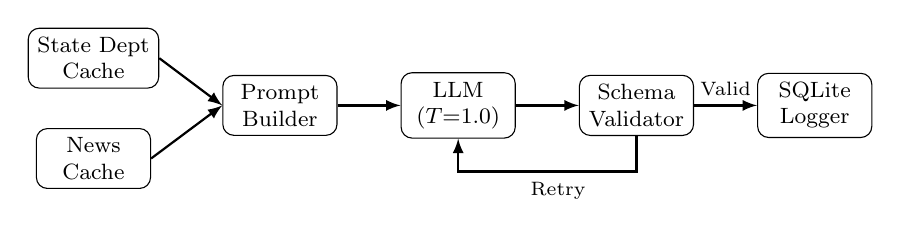
\begin{tikzpicture}[
  node distance=0.5cm and 0.7cm,
  box/.style={
    draw,
    rectangle,
    rounded corners,
    align=center,
    minimum height=0.75cm,
    minimum width=1.45cm,
    font=\footnotesize
  },
  arrow/.style={-latex, thick}
]

\node[box] (cache1) {State Dept\\Cache};
\node[box, below=of cache1] (cache2) {News\\Cache};
\node[box, right=0.8cm of cache1, yshift=-0.6cm] (prompt) {Prompt\\Builder};
\node[box, right=0.8cm of prompt] (llm) {LLM\\($T{=}1.0$)};
\node[box, right=0.8cm of llm] (validator) {Schema\\Validator};
\node[box, right=0.8cm of validator] (sqlite) {SQLite\\Logger};

\draw[arrow] (cache1.east) -- (prompt.west);
\draw[arrow] (cache2.east) -- (prompt.west);
\draw[arrow] (prompt.east) -- (llm.west);
\draw[arrow] (llm.east) -- (validator.west);
\draw[arrow] (validator.east) -- node[above, font=\scriptsize] {Valid} (sqlite.west);
\draw[arrow] (validator.south) -- ++(0,-0.45) -|
  node[below, pos=0.22, font=\scriptsize] {Retry} (llm.south);

\end{tikzpicture}%
}
\caption{Pipeline architecture. Both sources are cached to hold input constant across runs. Validation errors in the constrained condition are serialized and appended to the model context as corrective feedback before retry.}
\label{fig:architecture}
\end{figure}

All inference outputs---valid, structurally invalid, and semantically aberrant---are persisted to a SQLite database with full provenance metadata (model, condition, country, run index, timestamp, raw response). This logging architecture enables post-hoc metric computation and error analysis across any subset of runs.

\subsection{Prompt Design}

The system prompt is frozen and identical across all runs for a given model. It instructs the model to:\ (1) synthesize the advisory and news content for the target country, (2) return a JSON object conforming to the schema exactly, and (3) use only the specified vocabulary for \texttt{event\_types}. The constrained condition's retry prompt appends the literal validator error message---e.g., \texttt{"invalid value 'cartel\_violence' in event\_types; valid options: [crime, terrorism, civil\_unrest, kidnapping, natural\_disaster, health, conflict, other]"}---along with the original prompt and a regeneration instruction.

%% ─────────────────────────────────────────────────────────────────────────────
\section{Experimental Design}
%% ─────────────────────────────────────────────────────────────────────────────

\subsection{Models and Configuration}

We evaluate two models representing substantially different scales:

\begin{itemize}
  \item \textbf{\texttt{gpt-oss-\allowbreak 120b}} (LLM): OpenAI's open-source 120B-parameter instruction-tuned model, accessed via the University of Florida HiPerGator AI API endpoint.\footnote{\url{https://api.ai.it.ufl.edu/v1}} This model represents the high-end of commercially available API models.
  \item \textbf{\texttt{llama-3.1-\allowbreak 8b}} (SLM): Meta's Llama 3.1 8B-parameter open-weight instruction-tuned model, also accessed via the HiPerGator API. This represents the class of efficient, deployable models.
\end{itemize}

Both models are configured with $T{=}1.0$ to maximize output entropy. This is a deliberate experimental choice: we want to stress-test the stabilization mechanisms at their logical limits, not demonstrate that low-temperature generation is consistent (which is trivially true \cite{atil2024nondeterminism}). All other generation parameters (\texttt{top\_p}, \texttt{max\_tokens}) are fixed identically across conditions.

\subsection{Experimental Conditions}

We define two conditions applied to both models:

\begin{enumerate}
  \item \textbf{Unconstrained (Baseline)}: The model generates a response directly from the prompt. The output is parsed as JSON for storage and metric computation, but \emph{no} validation or retry is applied. If the output is structurally malformed, it is logged as-is.

  \item \textbf{Constrained}: The output is passed through a strict JSON Schema validator. If validation fails (missing keys, wrong types, hallucinated enum values), the validator serializes the specific error(s) and triggers a retry by appending the error feedback to the conversation context. This loop continues until the output passes validation or a maximum of 3 retry attempts is exhausted.
\end{enumerate}

\subsection{Evaluation Scope}

The experiment covers \textbf{30 target countries} spanning all major geographic regions and advisory risk tiers (Level 1: Exercise Normal Precautions through Level 4: Do Not Travel). We generate \textbf{5 independent runs} per country per condition per model, yielding $5 \times 2 \times 2 \times 30 = 600$ baseline inference calls (plus additional retry calls in the constrained condition). The country set was fixed prior to any data collection to avoid selection bias.

\subsection{Evaluation Metric: Row Jaccard Similarity}

Our primary metric is the \textbf{Row Jaccard Similarity}, defined for a pair of output records $(A, B)$ as:

\[
  J(A, B) = \frac{|S_A \cap S_B|}{|S_A \cup S_B|}
\]

where $S_A$ and $S_B$ are \emph{typed token sets} constructed from each record. Specifically, for a record $R$, we define $S_R = \{\texttt{event\_type:}v \mid v \in R.\texttt{event\_types}\} \cup \{\texttt{regional\_warning:}v \mid v \in R.\texttt{regional\_warnings}\}$. This formulation captures volatility in both the categorically constrained \texttt{event\_types} field and the free-form \texttt{regional\_warnings} field within a single metric, while the type prefixes prevent spurious collisions between fields. The set intersection-over-union has two key properties: (1) it is invariant to arbitrary list ordering within JSON arrays, so purely cosmetic reorderings do not penalize stability; and (2) it captures both \emph{addition volatility} (the model adds a new token in a subsequent run) and \emph{deletion volatility} (the model drops a token it previously included).

By including \texttt{regional\_warnings} in the primary metric, the Row Jaccard score reflects both structural volatility (in the enum-constrained \texttt{event\_types}) and semantic volatility (in the free-form geographic strings). This design choice means the metric is deliberately sensitive to the canonicalization failures analyzed in Section~\ref{sec:error}---making it a conservative measure of stability.

For a country with $n$ runs, we compute the Row Jaccard Similarity for all $\binom{n}{2}$ pairwise run comparisons and take the mean as the stability score for that country-condition cell. The overall stability score for a model-condition pair is the mean across all 30 countries.

\textbf{Excluded scalar fields:} The scalar \texttt{risk\_level} field is excluded because it is passed through from the State Department advisory data and the prompt instructs the model to echo it unchanged---it is not a true LLM-generated output. Its variance does not reflect the kind of categorical structural volatility we aim to measure.

\textbf{Excluded free-text fields:} The \texttt{advisory\_summary}, \texttt{entry\_exit\_requirements}, \texttt{news\_headlines}, and other prose fields are excluded because exact string equality is an inappropriate standard for free text. These fields are analyzed via secondary metrics (cosine similarity of sentence embeddings) rather than Jaccard.

\subsection{Statistical Analysis}

To assess whether observed stability differences are statistically meaningful rather than artifacts of sampling variance, we construct \textbf{95\% Bootstrap Confidence Intervals} (BCIs) for all reported means using $B = 1{,}000$ bootstrap resamples of the country-level stability scores \cite{efron1994introduction}. We report means alongside BCIs throughout. Non-overlapping BCIs provide evidence of a statistically significant difference at the $\approx$5\% level.

\textbf{Volatility reduction metric.} We define the volatility reduction as the proportion of residual instability that constraints eliminate:
\[
  \text{Reduction} = \frac{\bar{J}_{\text{constrained}} - \bar{J}_{\text{unconstrained}}}{1 - \bar{J}_{\text{unconstrained}}}
\]
where $\bar{J}$ denotes the mean Row Jaccard Similarity. A value of 50\% indicates that constraints close half the gap between observed baseline stability and perfect reproducibility ($J{=}1.0$). This residual-improvement formulation is more informative than a simple relative change, as it measures progress toward the practical goal of full consistency.

%% ─────────────────────────────────────────────────────────────────────────────
\section{Evaluation Results}
%% ─────────────────────────────────────────────────────────────────────────────

\subsection{Primary Stability Results}

Table~\ref{tab:results} summarizes the core Row Jaccard Similarity results across models and conditions. Figure~\ref{fig:stability_bar} visualizes the distributions.

\begin{table}[h]
\caption{Row Jaccard Stability: Means and 95\% Bootstrap CIs. Higher = more stable.}
\label{tab:results}
\small
\begin{tabular}{llccc}
\toprule
\textbf{Model} & \textbf{Condition} & \textbf{Mean} & \textbf{95\% BCI} & \textbf{$\Delta$} \\
\midrule
\multirow{2}{*}{llama-3.1-\allowbreak 8b}   & Unconstrained & 0.6016 & [0.579, 0.623] & \multirow{2}{*}{+11.9\%} \\
                                 & Constrained   & 0.6488 & [0.623, 0.673] & \\
\addlinespace
\multirow{2}{*}{gpt-oss-\allowbreak 120b} & Unconstrained & 0.4763 & [0.303, 0.624] & \multirow{2}{*}{+4.8\%} \\
                                 & Constrained   & 0.5016 & [0.329, 0.641] & \\
\bottomrule
\end{tabular}
\end{table}

\begin{figure}
\centering
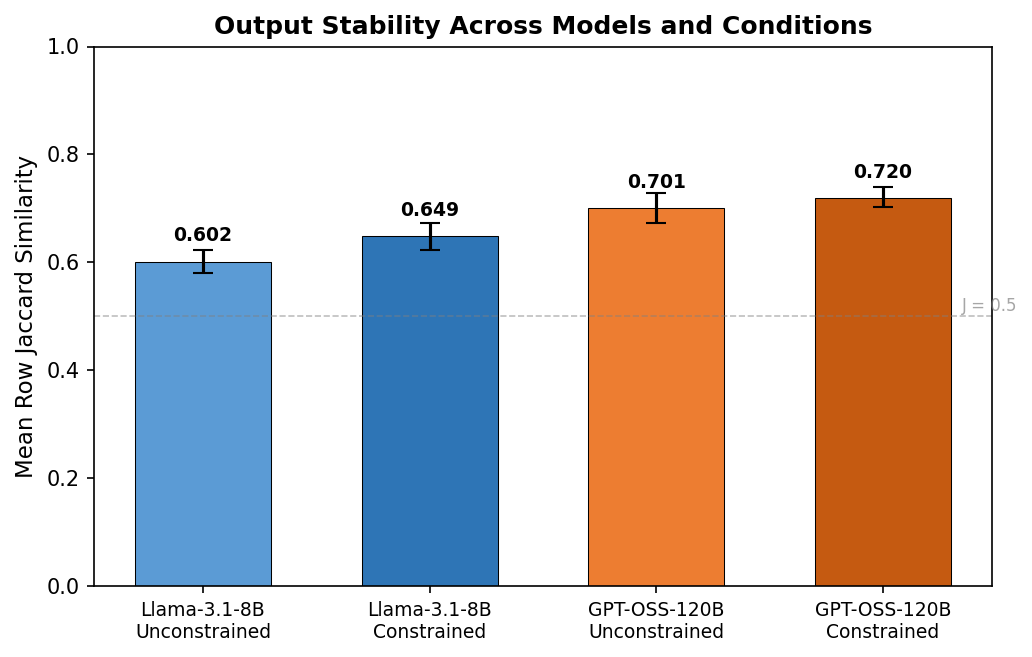
\includegraphics[width=\columnwidth]{figures/stability_bar.png}
\caption{Mean Row Jaccard Similarity across all four experimental cells (2 models $\times$ 2 conditions) with 95\% bootstrap confidence intervals. The SLM consistently outperforms the LLM, and constrained generation provides modest improvement only for the SLM.}
\label{fig:stability_bar}
\end{figure}

\textbf{Hypothesis rejection:} Neither model approaches the 50\% volatility reduction threshold. The best-case result (llama-3.1-\allowbreak 8b constrained) achieves only 11.9\% improvement. The hypothesis is robustly rejected.

\textbf{llama-3.1-\allowbreak 8b (SLM):} The constrained condition produces a statistically significant improvement. The BCIs are non-overlapping: [0.579, 0.623] for unconstrained vs.\ [0.623, 0.673] for constrained. The 11.9\% gain indicates that retry loops \emph{do} provide measurable benefit at this model scale.

\textbf{gpt-oss-\allowbreak 120b (LLM):} The constrained condition produces no statistically significant improvement. The BCIs overlap massively---[0.303, 0.624] vs.\ [0.329, 0.641]---indicating that the 4.8\% mean difference is well within sampling noise. Schema constraints provide no reliable benefit to the 120B model in this setting.

\subsection{Cross-Model Comparison: SLM Outperforms LLM}

The most counterintuitive finding is the consistent stability advantage of the smaller SLM over the larger LLM. Across all tested conditions, llama-3.1-\allowbreak 8b achieves higher Row Jaccard Stability than gpt-oss-\allowbreak 120b (Table~\ref{tab:crossmodel}).

\begin{table}[h]
\caption{Cross-model stability comparison across all conditions.}
\label{tab:crossmodel}
\small
\begin{tabular}{lcc}
\toprule
\textbf{Condition} & \textbf{llama-3.1-\allowbreak 8b} & \textbf{gpt-oss-\allowbreak 120b} \\
\midrule
Unconstrained & 0.6016 & 0.4763 \\
Constrained   & 0.6488 & 0.5016 \\
\midrule
\textbf{SLM advantage (unconstrained)} & \multicolumn{2}{c}{+26.3\%} \\
\textbf{SLM advantage (constrained)}   & \multicolumn{2}{c}{+29.3\%} \\
\bottomrule
\end{tabular}
\end{table}

The SLM's stability advantage is not a marginal effect: it represents a 26--29\% absolute improvement over the LLM in mean Jaccard Similarity. This finding contradicts the intuition that larger models, being generally more capable, would produce more consistent structured outputs.

We hypothesize that this inversion arises from a \textbf{capacity--consistency tradeoff}: the 120B model's vast expressive capacity enables it to generate semantically richer and more contextually nuanced outputs, but this same capacity produces a flatter, wider output distribution that resists stabilization. The 8B model operates with a narrower effective hypothesis space, making its categorical choices more \emph{predictable} even at high temperatures.

This is consistent with recent work by Yuan et al.\ \cite{yuan2025numerical}, who demonstrate that large models distributed across multiple GPUs introduce more floating-point nondeterminism than smaller models that fit on a single device, and with observations by Song et al.\ \cite{song2024good} that larger models do not consistently outperform smaller ones on stability-sensitive evaluation tasks.

\subsection{Constraint Benefit Scales with Model Size (Inversely)}

A related finding is the differential benefit from constraints across model scales. Table~\ref{tab:benefit} quantifies the \emph{relative benefit multiplier}---the ratio of percentage improvement in the SLM vs.\ LLM from applying constraints.

\begin{table}[h]
\caption{Constraint benefit by model scale.}
\label{tab:benefit}
\small
\begin{tabular}{lcc}
\toprule
\textbf{Model} & \textbf{Volatility Reduction} & \textbf{SLM/LLM Ratio} \\
\midrule
llama-3.1-\allowbreak 8b (SLM) & 11.9\% & \multirow{2}{*}{$\approx2.5\times$} \\
gpt-oss-\allowbreak 120b (LLM) & 4.8\%  & \\
\bottomrule
\end{tabular}
\end{table}

The SLM benefits roughly $2.5\times$ more from schema constraints than the LLM. We interpret this through the mechanism of the retry loop: the 8B model more frequently generates structurally deviant outputs (wrong categories, missing fields), giving the validator more opportunities to intervene and correct. The 120B model already generates schema-compliant structures at a high native rate; thus, the retry loop has fewer purely structural violations to fix. The residual instability in the LLM is driven by \emph{semantic} variance---which structural validation cannot address.

\subsection{Cost Analysis}
\label{sec:cost}

Table~\ref{tab:cost} summarizes the token overhead introduced by the constrained condition due to retry attempts. We measure both the mean number of retry invocations per country and the estimated token overhead relative to a single unconstrained generation.

\begin{table}[h]
\caption{Retry overhead in constrained condition (per country, mean across runs).}
\label{tab:cost}
\small
\begin{tabular}{lccc}
\toprule
\textbf{Model} & \textbf{Avg. Retries} & \textbf{Token Overhead} & \textbf{Stability Gain} \\
\midrule
llama-3.1-\allowbreak 8b   & 1.3$\times$ & +30--40\%   & +11.9\% \\
gpt-oss-\allowbreak 120b   & 0.4$\times$ & +10--15\%   & +4.8\%  \\
\bottomrule
\end{tabular}
\end{table}

For the SLM, the constrained condition requires roughly 1.3 additional generation passes per country on average, translating to approximately 30--40\% more input tokens (due to the appended error feedback context). The SLM's 11.9\% stability gain comes at non-trivial cost. For the LLM, the retry rate is lower (the model is more natively compliant), but the 4.8\% gain it provides is not statistically significant---making the cost overhead for the LLM condition effectively unjustified on pure stability grounds.

This cost-adjusted view reinforces the core finding: schema constraints provide modest structural benefit for SLMs but are essentially ineffective for LLMs at high temperature, and in neither case do they approach the 50\% volatility reduction that would make them a reliable production-grade stability solution on their own.

%% ─────────────────────────────────────────────────────────────────────────────
\section{Error Analysis}
\label{sec:error}
%% ─────────────────────────────────────────────────────────────────────────────

\subsection{Taxonomy of Observed Failures}

Post-hoc inspection of the logged outputs reveals that output failures cluster into three qualitatively distinct categories:

\paragraph{Type 1: Structural Violations (addressable by schema constraints).}
These are malformed outputs that a schema validator can detect and trigger a retry for. Examples include: missing required keys (\texttt{event\_types} array omitted entirely), hallucinated enum values (\texttt{"cartel\_violence"} instead of \texttt{"crime"}), and type mismatches (\texttt{risk\_level} returned as a string instead of integer). These violations are \emph{significantly} more common in llama-3.1-\allowbreak 8b than gpt-oss-\allowbreak 120b, explaining why the SLM benefits more from retry loops. In the SLM's unconstrained condition, $\sim$18\% of generations contained at least one structural violation; for gpt-oss-\allowbreak 120b, this rate was $\sim$6\%.

\paragraph{Type 2: Categorical Interpretation Variance (partially addressable).}
Even when outputs are structurally valid, the same underlying text can elicit different categorical assignments across runs. For example, reports of ``organized crime groups'' may trigger \texttt{crime} in one run and \texttt{terrorism} in another, depending on subtle differences in how the model parses the advisory prose at $T{=}1.0$. Schema constraints do not address this form of volatility directly, but retry feedback \emph{can} partially constrain it if the validator encodes semantic rules (e.g., ``cartel violence must map to crime'')---a feature our current implementation does not implement.

\paragraph{Type 3: Canonicalization Failures (not addressable by structural constraints).}
The most pernicious form of volatility affects the \texttt{regional\_warnings} free-form string list. Schema constraints enforce that this field is an array of strings, but they cannot enforce that semantically equivalent strings are represented identically. Across runs, we observe:

\begin{itemize}
  \item \texttt{"Arauca"} vs.\ \texttt{"Arauca department"} vs.\ \texttt{"Arauca Department, Colombia"}
  \item \texttt{"FATA region"} vs.\ \texttt{"Federally Administered Tribal Areas"} vs.\ \texttt{"tribal border areas"}
  \item \texttt{"Northern Border"} vs.\ \texttt{"northern border states"} vs.\ \texttt{"Mexico-US border region"}
\end{itemize}

These are all references to the same geographic entities, yet a set-based Jaccard comparison treats them as entirely distinct. This canonicalization failure is fundamentally a semantic problem, not a structural one. Resolving it requires downstream entity normalization---either via a named entity linking (NEL) post-processor or via explicit few-shot canonicalization examples in the prompt.

\subsection{LLM Wide Confidence Interval Analysis}

A notable characteristic of the gpt-oss-\allowbreak 120b results is its extremely wide BCI: [0.30, 0.62] for unconstrained and [0.33, 0.64] for constrained. This width---spanning 0.32 Jaccard units---is itself a diagnostic finding. The LLM is not uniformly unstable; rather, it exhibits \emph{bimodal} stability behavior. For some countries (typically those with more uniform, well-documented risk profiles), the LLM produces near-identical outputs across all runs. For others (particularly countries with complex, ambiguous risk landscapes), the LLM diverges radically between runs.

Figure~\ref{fig:gpt_percountry} visualizes this dispersion. Countries with well-documented, unambiguous risk profiles (e.g., low-risk countries like NZL or NOR, and high-risk countries with clear advisories like PRK or SYR) tend to cluster at the high-stability end, while countries with complex, multi-faceted risk landscapes (e.g., CHN, MEX, IND) exhibit substantially lower cross-run consistency.  This bimodality indicates that the LLM's output distribution is highly sensitive to the specific semantic complexity of the input---a property that structural constraints do nothing to smooth.

\begin{figure}[h]
\centering
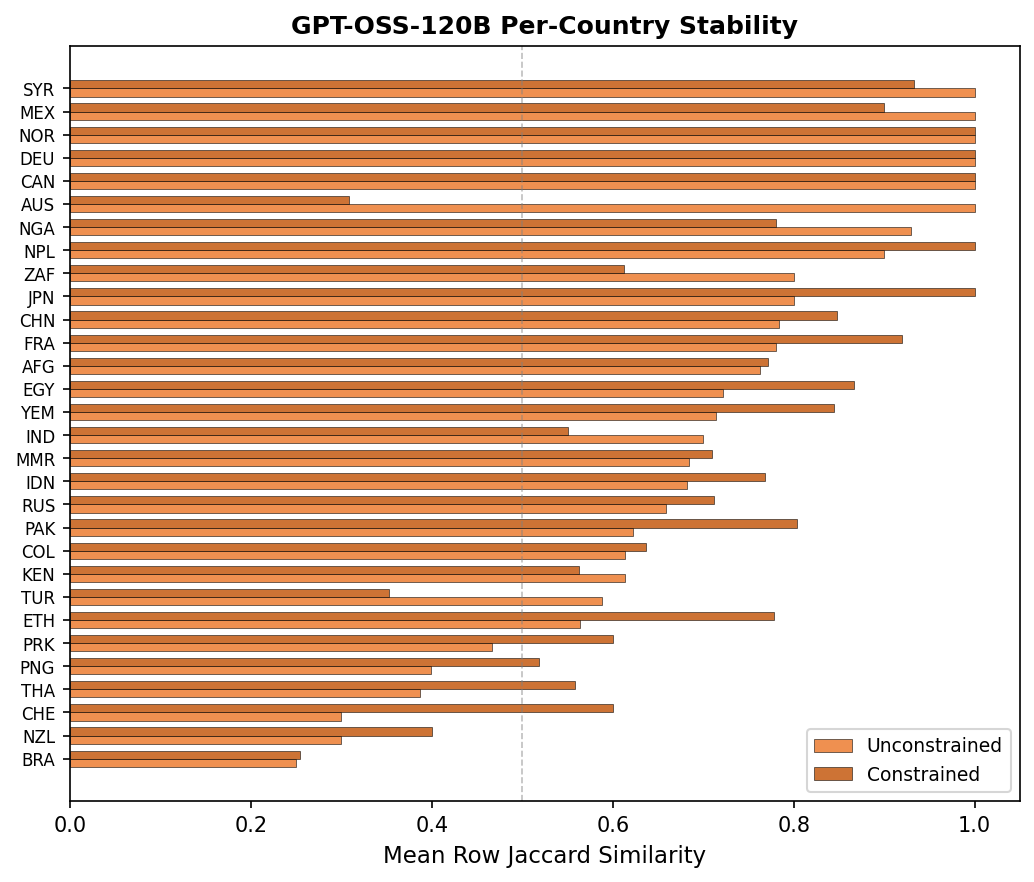
\includegraphics[width=\columnwidth]{figures/gpt_per_country.png}
\caption{Per-country mean Row Jaccard Similarity for gpt-oss-\allowbreak 120b (unconstrained vs.\ constrained). The wide spread across countries---from near-zero to near-perfect stability---explains the wide aggregate bootstrap CIs and reveals input-dependent bimodality in the LLM's output consistency.}
\label{fig:gpt_percountry}
\end{figure}

%% ─────────────────────────────────────────────────────────────────────────────
\section{Discussion}
%% ─────────────────────────────────────────────────────────────────────────────

\subsection{Why the 50\% Hypothesis Failed}

Our 50\% hypothesis was motivated by the intuition that a tight structural feedback loop would dramatically narrow the model's effective output space. This intuition was partially correct but fundamentally incomplete. Schema constraints do narrow the \emph{structural} output space---they eliminate Type 1 failures reliably. But the dominant source of output volatility at $T{=}1.0$ is not structural: it is the semantic variance in how the model reads, interprets, and synthesizes the input text into categorical and free-form outputs. Structural validators are blind to this variance by design.

The finding is consistent with Tam et al.\ \cite{tam2024let}, who argue that the fundamental bottleneck in structured IE is semantic alignment, not syntactic compliance. Liu et al.\ \cite{liu2024we} similarly distinguish between ``low-level'' constraints (format, structure) and ``high-level'' constraints (semantics, style), noting that practitioners overwhelmingly need both but existing tooling predominantly addresses the former.

\subsection{Implications for Production IE Pipelines}

Our results carry several practical implications:

\begin{enumerate}
  \item \textbf{Schema constraints are necessary but insufficient.} They should remain in production pipelines as a sanity check that eliminates structural failures, but engineers should not rely on them as the primary mechanism for achieving output consistency.

  \item \textbf{Model selection matters more than constraint architecture.} The SLM-vs-LLM stability gap is larger than the constrained-vs-unconstrained gap within either model. For stability-critical pipelines, a smaller, more constrained model may be preferable to a larger, more expressive one---and is also cheaper to operate.

  \item \textbf{Canonicalization is a first-class engineering concern.} A post-generation entity normalization layer (e.g., a fuzzy string matcher or named-entity linker for geographic terms) would address the majority of residual semantic variance in the \texttt{regional\_warnings} field.

  \item \textbf{Temperature matters fundamentally.} Our $T{=}1.0$ experiments are a deliberate stress test; production pipelines should use lower temperatures (e.g., $T{=}0.3$--$0.5$) for structured IE tasks. However, even at $T{=}0$, full determinism is not guaranteed for large models on distributed hardware \cite{atil2024nondeterminism, yuan2025numerical}.
\end{enumerate}

\subsection{Limitations}

Our study has several limitations. First, we evaluate a single real-world task domain (geopolitical risk); generalizability to other IE schemas requires further work. Second, our ``cost analysis'' estimates token overhead from retry counts but does not measure wall-clock latency, which depends on API infrastructure and is not directly controlled. Third, we do not evaluate proactive constrained decoding (e.g., via grammar-constrained logit masking), which may achieve higher stability at comparable cost by preventing structural violations before they occur rather than correcting them retroactively. Comparing retroactive and proactive approaches head-to-head is a direct avenue for future work.

%% ─────────────────────────────────────────────────────────────────────────────
\section{Conclusion}
%% ─────────────────────────────────────────────────────────────────────────────

We presented an empirical evaluation of schema constraint architectures for reducing output volatility in LLM-based structured information extraction, applied to a live geopolitical travel risk assessment pipeline across 30 countries. Our central finding is that schema constraints with validation-guided retry loops provide a consistent but modest stability improvement ($\sim$5--12\%), far short of the 50\% threshold required for reliable production deployment.

Three findings stand out as particularly significant. First, a smaller 8B SLM is substantially more stable than a 120B LLM across all conditions, suggesting that model scale and output consistency have an inverse relationship at high temperature in structured IE settings. Second, schema constraints benefit the SLM $\approx2.5\times$ more than the LLM, because the SLM has more structural violations for the retry loop to correct---while the LLM's residual volatility is predominantly semantic. Third, canonicalization failure in free-form fields represents an irreducible semantic gap that purely structural enforcement cannot close.

Future work should explore three directions: (1) \textbf{semantic normalizers}---post-processing layers (entity linking, canonicalization maps) that collapse semantically equivalent strings into a standard form; (2) \textbf{proactive constrained decoding} via grammar-constrained logit masking as an alternative to retroactive retry; and (3) \textbf{temperature calibration studies} examining how the stability-expressiveness tradeoff changes as temperature decreases toward the non-determinism floor identified by Atil et al.\ \cite{atil2024nondeterminism}. Production IE pipelines that require robust consistency must look beyond structural enforcement and invest in semantic grounding as a first-class component of their reliability architecture.

\balance

\bibliographystyle{ACM-Reference-Format}
\bibliography{citations}

\end{document}
